\documentclass[sigconf]{acmart}

\usepackage{hyperref}

%\usepackage{endfloat}
%\renewcommand{\efloatseparator}{\mbox{}} % no new page between figures

\usepackage{booktabs} % For formal tables

\settopmatter{printacmref=false} % Removes citation information below abstract
\renewcommand\footnotetextcopyrightpermission[1]{} % removes footnote with conference information in first column
\pagestyle{plain} % removes running headers


\begin{document}
\title{Big Data and Analytics in Blockchain}


\author{Ashok Kuppuraj}
\orcid{1234-5678-9012}
\affiliation{%
  \institution{Indiana University}
  \streetaddress{}
  \city{Bloomington} 
  \state{Indiana} 
  \postcode{43017-6221}
}
\email{akuppura@iu.edu}


% The default list of authors is too long for headers}
\renewcommand{\shortauthors}{G. v. Laszewski}


\begin{abstract}
Big data and its technologies help in augmenting and improving the current Blockchain technology and overcome the problems around it.
\end{abstract}

\keywords{i523, hid324, Big data, Blockchain, Cryptocurrency, Bitcoin, Transaction, Smart chain}


\maketitle

\DONE{Images are not in figure environment, se original template or other peoples papers}

\section{Introduction}
The objective is to concur the abilities of the two broad topics in the current technology world, Big Data, and Block Chain. Blockchain and Big data are still evolving technologies, which gives us enough opportunity to explore and invent new concepts for its own good. As these are still evolving, we can leverage one’s solution on the other. To leverage each one’s problems and solutions, we must first identify the similarities in two frameworks and how these similarities are related and what solution we are going to adopt.


\section{What is Big Data}

Big data can be described as any type of data with large volume, velocity, and variety \cite{vvv:online}. The history of Big data starts from the moment we started using computers back in the 1990s, however, we choose not to use all the generated data due to constraints in the processing and storage systems. Later, people understood that they are missing a lot of useful information to the business due to these constraints, and started leveraging data warehouse to process data in batch after data generation. At a certain point in time, even the data warehouse systems are not capable to handle the
volume and velocity of data, we are generating\cite{Bigdataintro} is exponential growth in data generation due to wide adoption of computers by humans in the form of mobile, PCs and introduction of IoT sensors, resulting in the need for technology to process these data and it is termed as "Big Data" \cite{datagrowth}.


\section{Block Chain}

 Blockchain can be defined as a decentralized, public ledger persisted in a connected set of immutable Blocks. The core idea is to perform any set of a transaction without a governing third-party avoiding double spending by Distributed consensus. A transaction happens with an entity called tokens, tokens are the actual digital asset of a blockchain. The implementation begins with an entity A initiating the transaction, an initiated transaction request from A to B is broadcasted with Gossip protocol to most of the nodes, the transaction is validated by miners with the ledger available with them, the validation includes checking digital signatures and the previous input to that entity (i.e current withholding). Later the validated transactions are grouped with reference to its previous address and added as a current block. This block is then broadcasted to the network and the network peers validate the block and add them to their ledger, confirming the transaction. Hence, termed as "Blockchain" \cite{Bitcoin}.

\section{Big data vs Blockchain}
As far as data is concerned, both Big data and Blockchain go in parallel.Both involve processing data at volume, velocity, and variety which is the basic evaluation factor for defining big data. In the below section, the analysis is made on how these three V's corresponds to Block Chain, with an example from Bitcoin, one of the front-runners in implementing Blockchain technologies.

\subsection{Data Volume}
Though the data volume share of blockchain is considerably low compared to current Big data average, the volume it generates in an overall network perspective in terms of network I/O, logs, transaction data, it fits well with the terms of big data. For example, consider the transaction growth of Bitcoin \cite{bitcointrans}, the volume of the transaction was averaging 5K in 2011, whereas in 2017 the average is 200K with an increase of 400 percent over 5 years and the volume is likely to grow in an exponential scale with the global acceptance of Blockchain technologies. 

\begin{figure}
  \centering
  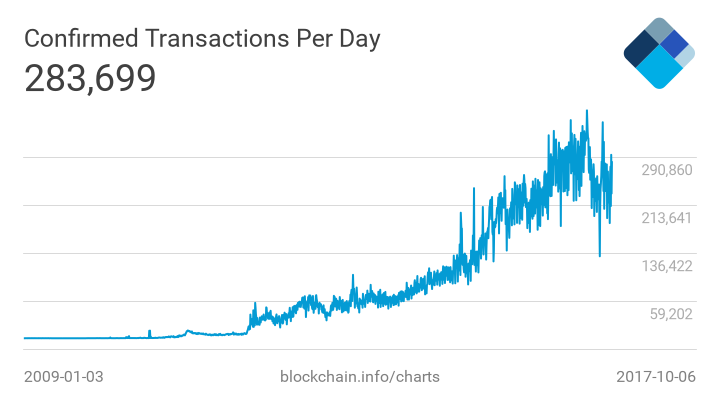
\includegraphics[width=1.0\columnwidth]{images/bitcoin-trans.png}
  \caption{The snippet describes the number of transactions, in Bitcoin's network } 
  \label{fig:Figure1} 
\end{figure}

\subsection{Data velocity}
In data terms, even 10 MB of data is considered huge when its getting generated within a span of seconds, hence we must consider the velocity as an important metric in analyzing the data, here in Blockchain, though the transactions are not of high volume, but other non-token transactions like Gossip calls, smart contract transfers, block transfers, acceptance protocol were happening every second, which in turns generate huge amount of data within 10 minutes of this interval with respect to Bitcoin.

\begin{figure}
  \centering
  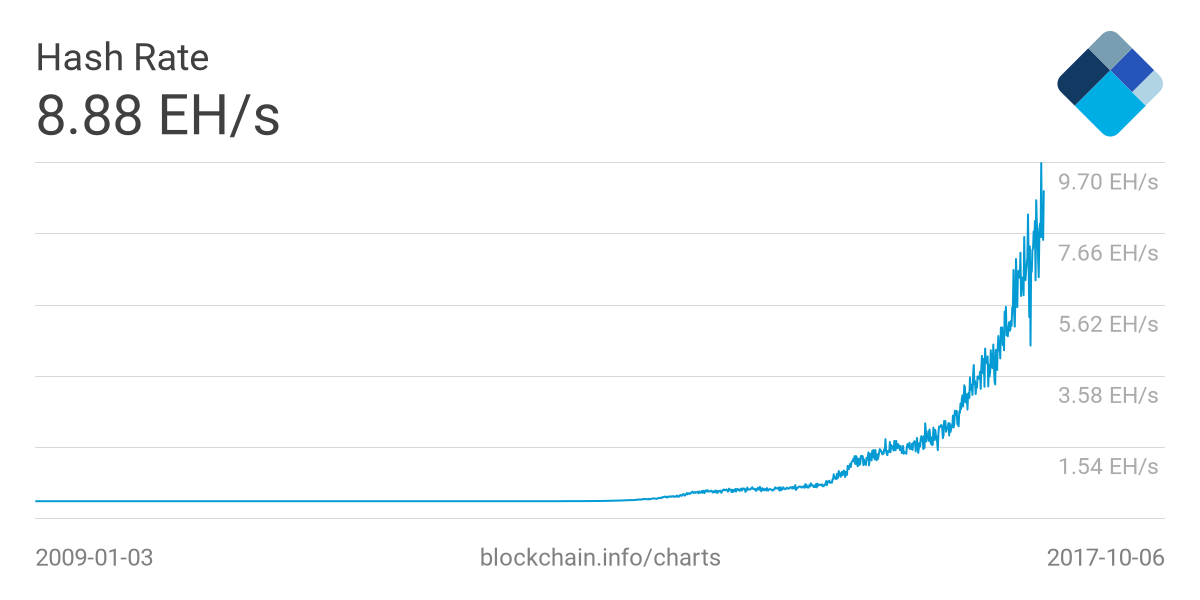
\includegraphics[width=1.0\columnwidth]{images/hash-rate.png}
  \caption{The snippet describes the number of hashes resolved per second, in Bitcoin's network \cite{hastratepersec}} 
  \label{fig:Figure2} 
\end{figure}

\subsection{Data Variety}
In a wide perspective, Blockchain deals with multiple varieties of structured data like Token data, Smart contracts, consensus data, logging data and unstructured data like videos \cite{livepeer-BC-stream}, audio depending upon the use-case of the Blockchain. And the popularity it has now and based on the current growth trend in the acceptance of decentralization, Blockchain technology will tend to generate more data in a wide range of varieties.

\section{Implementation - Big data technologies in Blockchain}
Before we start on the implementation of Big data technologies, its required to identify the problems Blockchain faces now in scope with Big data solutions, one of the main problems are slow transactions and visualization through complex analytic calculation. Though we have other problems, we consider the above two as the most important to enhance the success rate of this technology.For example, consider Bitcoin, the overall transaction timing is fewer in-terms of interbank transaction however for the end user it takes a minimum of 20 Min's to complete a transaction, whereas, in Visa, for instance, it can perform up to 24000 transactions per second \cite{Visa}.


\subsection{Transaction processing}
To deal with improving the transaction speed of a peer-to-peer network, first it is required to streamline the asynchronous process of gossip protocols, handshake between peers to increase the transaction processing speed, also by removing the block size limits\cite{Optimize-bitcoin} we can increase the frequency of the block building, this optimization can be easily achieved with the help of Big data queuing utilities like Apache Kafka by creating individual topics for each set of Broadcasting, Block Acknowledgement, and consensus sharing between peers,   and second is to increase the Hash processing capacity by horizontal scaling with the help of Apache Spark or Apache Flink. By using these open source tools for hash processing, it is not required to invest on high-value GPU's to process data.

For an instance, Kafka can handle up to 200,000 messages/second (220MB/second)\cite{kafka-performance}, which is way more than any other existing banking infrastructure can provide.

\subsection{Visualization}
The current visualization options available with blockchain is based on the shared ledger available in the network, to fetch the real-time reporting or visualizing the happenings in the network, one must have to take part in the network and share all the interactions and ledger details for any sort of analytic needs. As discussed in the previous section, if we start using Kafka for other peer-to-peer interactions via topics, we can seamlessly provide real-time reporting to users.

\subsection{Smart-Blockchain}
The next big leap in the Blockchain would be the implementation of Machine learning in the Blockchain. The current versions of blockchain don't have any machine learning modules or algorithm built along with. By including the machine learning modules in the blockchain network, Blockchain can be made smart by predicting malicious activities, optimizing transactions and evaluation of its sources.

\subsection{Data Persistence}
Storage is an important aspect of any platform, both in Big data and Blockchain, most of the data is persisted. In Blockchain, the data involving contracts and blocks are either stored in a file system or database \cite{Antonopoulos:2014:MBU:2695500}, e.g Google's LevelDB in Bitcoin Blockchain. In Big data, the data storage is in Hadoop's File System or a database. Both use the data storage for write once and read many as their retention strategy. When it comes to data persistence, fault tolerance and recovery cannot be left behind. In big data technologies like Hadoop, the fault tolerance is ensured by HDFS, with the help of replication and Journal Managers. Whereas in Blockchain, the same has been ensured with Merkle tree data structure simulating Journal manager through validation and peer-to-peer network which simulates nodes of replication. 

\subsection{Decentralization}
Decentralization can be defined as a distribution of functions or power\cite{Dictionery}, decentralization can be modeled in every stage of an application's lifecycle. In terms of data processing, data decentralization considers the data stays where it gets generated and the analytic happens at the same place. In large organizations, each unit independently generates data, process and analyze it without impacting the others. consider if it is a centralized system, the flexibility of each unit has to be constrained and output has to be generalized or standardized at the organization level, this seriously impacts the evolving needs of each units\cite{IsDataDe19:online}. Hence decentralization can be a good approach in order to cope with the changing world. However, the changes cannot be easily incorporated with conventional technologies like ETL (Extract-Transform-Load) tools and mainframe which runs based on fixed terms, the big data technologies come into rescue with the schema-less data model, distributed file system, etc.

Both Big data technologies and Blockchain technologies go hand in hand with decentralization. Let's consider in a view of data processing, In Apache Hadoop framework the data is processed locally in the individual nodes whereas in Informatica the data is transferred to centralized servers to perform any processing\cite{Informat9:online}. In Blockchain, the hash processing happens in the peer nodes instead of a centralized server and shared with the other peers for validation and acceptance.


\section{Conclusion}
Although Blockchain provides a solution for Real life problems, it would be nearly impossible without its implementations leaning towards Big data solutions. Big data and its technologies is a front-runner in the handling of data of different volume, velocity, and variety which Blockchain is yet to reach. With the current acceptance rate of Blockchain, Big data, and Machine learning technologies, maybe in future, countries don't need a leader to take decisions on their behalf, people can collectively take a state decision and election process will be so simple that it can happen every day.


\begin{acks}

  The author would like to thank Dr. Gregor von Laszewski for his
  support and suggestions to write this paper.

\end{acks}

\bibliographystyle{ACM-Reference-Format}
\bibliography{report} 

\end{document}
  